% SPDX-FileCopyrightText: 2023 SAP SE
%
% SPDX-License-Identifier: Apache-2.0
%
% This file is part of FEDEM - https://openfedem.org

%%%%%%%%%%%%%%%%%%%%%%%%%%%%%%%%%%%%%%%%%%%%%%%%%%%%%%%%%%%%%%%%%%%%%%%%%%%%%%%%
%
% FEDEM User Guide.
%
%%%%%%%%%%%%%%%%%%%%%%%%%%%%%%%%%%%%%%%%%%%%%%%%%%%%%%%%%%%%%%%%%%%%%%%%%%%%%%%%

\Section{Triads}{triads}

\IconTextFirst{triad}{To construct a working mechanism, parts and/or beams are
  connected to each other using elements such as joints, springs and dampers.
  Fedem uses a modeling object called a {\sl triad} to make these connections.
  Triads are also used as attack point for external point loads on parts,
  and concentrated additional masses.
  The triad defines a set of three mutually perpendicular coordinate axes
  originating from the connection point.}

Triads enable parts to be connected to other mechanism elements using
the parts' FE nodes as connection points. When parts are joined together
in your model, the connection points are retained after the model
reduction process as external FE nodes
(see the \FedemTGuide{Chapter 3, "Model Reduction"}).
During simulation, a triad must move rigidly in translation and
rotation with the FE node to which it is attached. This means that
triads (and therefore connections) can only be placed on FE nodes with
six DOFs, since three-DOF solid nodes allow random rotation.


%%%%%%%%%%%%%%%%%%%%%%%%%%%%%%%%%%%%%%%%%%%%%%%%%%%%%%%%%%%%%%%%%%%%%%%%%%%%%%%%
\SubSection{Triads in joints}{triads-in-joints}

Triads are used to connect joints to parts and beams in the model in the
same way that a door hinge uses one hinge-plate to attach the hinge to
the door and the other to attach the hinge to the frame. Each type of
joint may use a different number of triads to make the required
connections. When a joint is created, its triads are created along, and
positioned automatically (see \refSection{joints}{Joints} for more
information about how triads are used in joints).


%%%%%%%%%%%%%%%%%%%%%%%%%%%%%%%%%%%%%%%%%%%%%%%%%%%%%%%%%%%%%%%%%%%%%%%%%%%%%%%%
\SubSection{Triad symbols}{triad-symbols}

Because triads can be used for several different purposes---as building
blocks for joints; attachment points for springs, dampers, and loads;
and measuring points for sensors---different symbols are used to
visualize the triads based on its usage.

\Tip{When attached, all triads are the same color, regardless of the symbol used
  to represent them. To identify a triad, simply look for the triad color
  (default green) (Click the \textbf{General Appearance} button to access
  options for changing the color of triads and other mechanism elements).}

\clearpage
\noindent
\begin{minipage}{0.6\textwidth}
  \raggedright

\subsubsection{Diamond}

A triad is depicted as a small diamond (shown at right) when the triad's
{\sl coordinate system} is {\sl not} used in your mechanism---for example,
when a triad is placed on an FE node and no other mechanism element is attached,
or when it is only used to attach a load, torque, axial spring, or damper.

\subsubsection{Coordinate system}

A triad is visualized as a coordinate system (shown at right) when the triad
stands alone, and its coordinate system is referenced in one of the
following ways:
\end{minipage}%
\begin{minipage}{0.4\textwidth}
  \raggedleft
  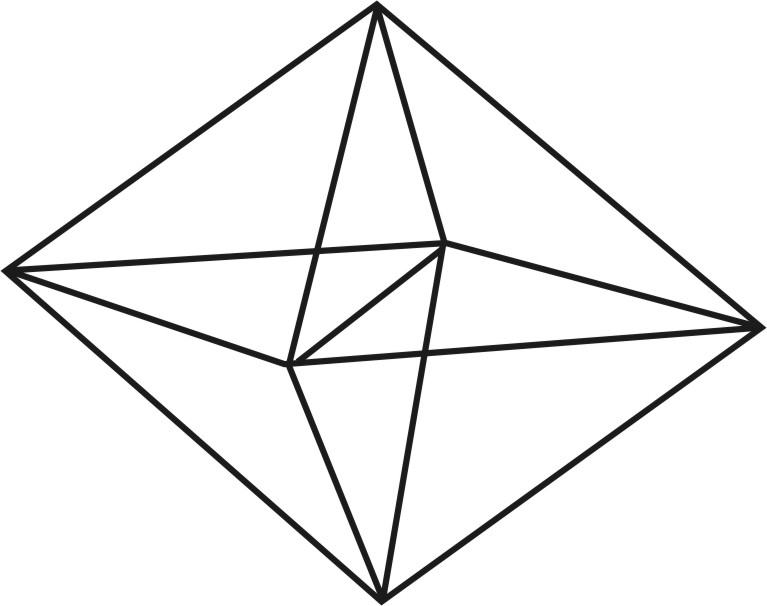
\includegraphics[scale=0.4]{Figures/DiamondRedo} \\[10mm]
  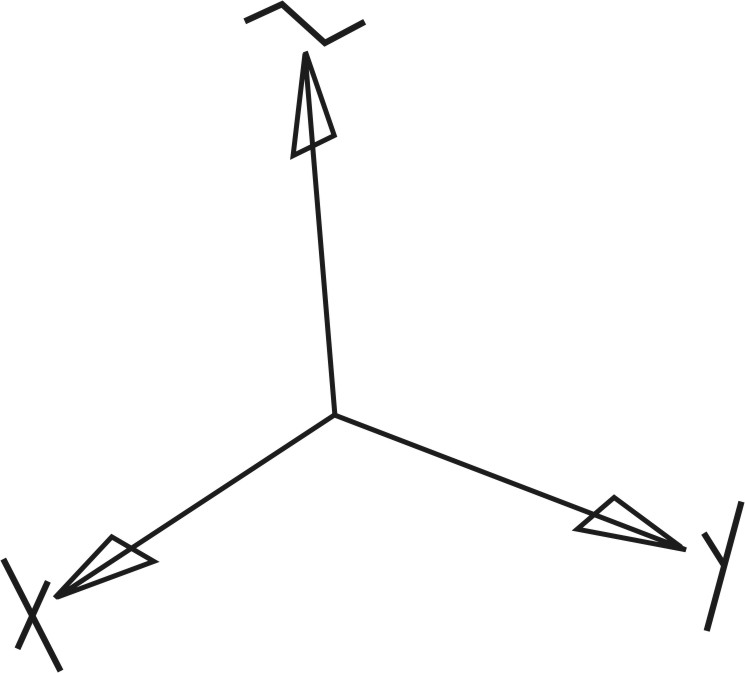
\includegraphics[scale=0.4]{Figures/CoordinateSystem}
\end{minipage}

\medskip
\begin{itemize}
\item
  The triad's coordinate system is used by a sensor to  measure a variable with
  components defined in the local (triad) coordinate system
  (see \refSection{sensors}{Sensors}).
\item
  The triad's coordinate system is used to define mass or inertia components
  for the triad (see \refSection{triad-properties}{Triad properties} below).
\item
  The triad's coordinate system is used to define boundary conditions for use
  in the initial equilibrium analysis and/or the system eigenvalue analysis
  (see \refSection{triad-properties}{Triad properties} below).
\end{itemize}

\subsubsection{Member of a Joint}

The triads that are members of joints are visualized as integral parts of the
different joint symbols. Refer to \refSection{joints}{Joints} for details.


%%%%%%%%%%%%%%%%%%%%%%%%%%%%%%%%%%%%%%%%%%%%%%%%%%%%%%%%%%%%%%%%%%%%%%%%%%%%%%%%
\SubSection{Triad properties}{triad-properties}

To view the properties of a triad, select it in the {\sl Modeler} view or Model
Manager {\sl Objects} list. The Property Editor panel for a triad consists of
six tabs for the triad DOFs where their properties are displayed in detail,
in addition to the {\sl General} (shown below), {\sl Origin}
and {\sl Results} tabs.

\begin{figure}[H]
  \begin{picture}(343,93)
    \put(0,0){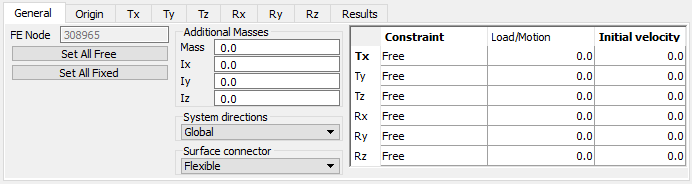
\includegraphics[width=\textwidth]{\ReferenceImg/prp/triad-1}}
    \put(65,69){\Bullet{1}}
    \put(140,70){\Bullet{2}}
    \put(140,20){\Bullet{3}}
    \put(140,3){\Bullet{4}}
    \put(225,73){\Bullet{5}}
    \put(65,55){\Bullet{6}}
    \put(40,88){\Bullet{7}}
    \put(110,88){\Bullet{8}}
    \put(173,88){\Bullet{9}}
  \end{picture}
\end{figure}

\begin{bulletlist}
\item{\sl FE Node} -- This field
  displays the ID number of the FE node to which the selected triad is attached.

\EnumTip{The FE node number can be useful if you edit the part \File{.ftl} file
  manually (described in \refAppendix{fe-model-interface}{FE Model Interface}).}

\item{\sl Additional Masses} --
  These fields enable you to apply additional mass and inertia to the triad.

\item{\sl System directions} --
  This pull-down menu enables selecting different reference coordinate systems
  for the DOFs associated with the triad.
  \vskip-3mm
  \begin{itemize}
  \subitem{\sl Global} :
    The global inertial coordinate axes are used.
  \subitem{\sl Local, initial} :
    The local axis directions of the triad's modeling configuration are used.
  \subitem{\sl Local, withrotated} :
    The local axis direction of this triad that follows the deformation
    of the model during simulation are used.
  \end{itemize}

\item{\sl Surface connector} --
  If the triad has a surface connector associated with it
  (see \refSection{surface-connectors}{Surface Connectors}), you may here
  switch the connector type between {\sl Flexible} and {\sl Rigid}.

\item{\sl Summary table} --
  An overview of all the DOF properties in the triad is provided here.
  This table is for viewing only (can not be edited).
  \begin{itemize}
  \subitem{\sl Constraint} :
    Shows the {\sl Constraint type} selected for this triad DOF.
  \subitem{\sl Load/Motion} :
    Shows the applied load or prescribed motion.
  \subitem{\sl Initial velocity} :
    Shows the initial velocity at this triad DOF.
  \end{itemize}

\item{\sl Set All Free/Fixed} --
  These two buttons (not present for slave triads) enable you to quickly set the
  Constraint type of all triad DOFs to either {\sl Free} or {\sl Fixed},
  without the need to go into each of the DOF tabs.

\item{\sl Origin} --
  This tab contains the {\sl Origin properties} of the triad.
  See \refSection{origin-property}{Origin property}.

\item{\sl Triad DOF tabs} --
  This tabs display the detailed properties related to each of the six DOFs
  associated with the triad. The available options here depends on the selected
  {\sl Constraint type}, as shown below.

\item{\sl Results} --
  This tab contains toggles for activating output of certain solution variables
  related to the triad, see
  \protect\hyperlink{triad-results-tab}{\sl"Results tab"} below.
\end{bulletlist}


\SubSubSection{Free DOF}{free-dof}

\begin{figure}[!h]
  \begin{picture}(343,80)
    \put(0,0){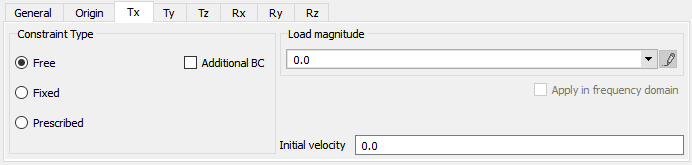
\includegraphics[width=\textwidth]{\ReferenceImg/prp/triad-3}}
    \put(190,48){\Bullet{1}}
    \put(250,33){\Bullet{2}}
    \put(220,5){\Bullet{3}}
    \put(75,46){\Bullet{4}}
  \end{picture}
\end{figure}

\begin{bulletlist}
\item{\sl Load magnitude} --
  You can apply a load in this triad DOF. This will be a torque or a force
  depending on whether this is a translational or a rotational DOF.

\item{\sl Apply in frequency domain} --
  If a {\sl Function} is specified in the {\sl Load magnitude} field,
  this toggle will enable the load to be applied in the frequency domain
  instead of the time domain, if the {\sl Frequency response analysis} toggle
  is enabled in the Dynamics Solver Setup dialog box, see
  \refSection{dynamics-solver-basic-mode}{Dynamics Solver (Basic Mode)}.

\item{\sl Initial velocity} --
  You may specify a velocity that should be applied as initial condition in this
  DOF, i.e., the actual velocity at the start time of the dynamics simulation.

\item{\sl Additional BC} --
  When this toggle is enabled, the movement in this DOF is fixed during the
 initial equilibrium analysis and optionally also in the eigenmode analysis.
 (See also
  \refSubSection{eigenmode-tab}{Eigenmode tab}{dynamics-solver-advanced-mode},
  and the \FedemTGuide{Section 7.8, "Quasistatic equilibrium"}
  and {\sl Section 9.6, "Eigenvalue results"}.)
\end{bulletlist}

\Tip{Sometimes during the creation of a complex model, it is useful to test
  the dynamics when all initial conditions are off (equal to zero).
  To facilitate this without having to manually remove all the defined initial
  conditions, the dynamic solver option {\tt -ignoreIC} may instead be specified
  in the Additional Solver Options dialog box (in the Dynamics Solver field,
  see \refSection{additional-solver-options}{Additional solver options}).
  Then all defined initial conditions will be ignored (assumed zero).}


\subsubsection{Fixed DOF}

\begin{figure}[H]
  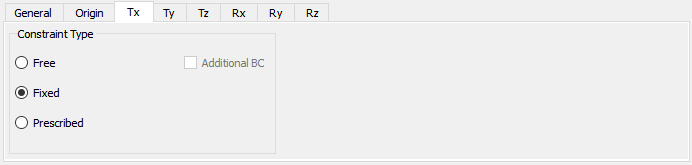
\includegraphics[width=\textwidth]{\ReferenceImg/prp/triad-4}
\end{figure}

For Fixed triad DOFs, no further property settings are available.

\Tip{You may plot the reaction force associated with a fixed or prescribed
  triad DOF by selecting the {\rm Force} or {\rm Moment} item under the Triad
  node in question from the RDB selector (see
  \refSubSection{selecting-rdb-results}{Selecting RDB results}
                {curve-properties}).}


\SubSubSection{Prescribed DOF}{prescribed-dof}

\begin{figure}[H]
  \begin{picture}(343,80)
    \put(0,0){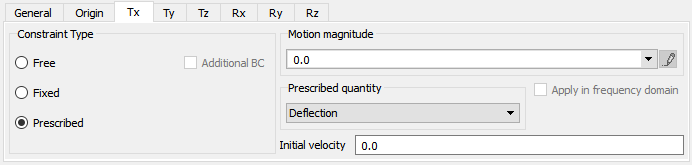
\includegraphics[width=\textwidth]{\ReferenceImg/prp/triad-5}}
    \put(170,48){\Bullet{1}}
    \put(190,21){\Bullet{2}}
    \put(266,22){\Bullet{3}}
    \put(220,5){\Bullet{4}}
  \end{picture}
\end{figure}

\begin{bulletlist}
\item{\sl Motion magnitude} --
  You can prescribe a constant deflection, velocity or acceleration by typing
  the desired value into this field, or a time-dependent evolution of the motion
  by selecting a function.

\item{\sl Prescribed quantity} --
  You may choose whether you want to prescribe the {\sl Deflection},
  the {\sl Velocity} or the {\sl Acceleration} for the triad DOF.

\item{\sl Apply in frequency domain} --
  If a {\sl Function} is specified in the {\sl Motion magnitude} field,
  this toggle will enable the prescribed motion to be applied in the frequency
  domain instead of the time domain, if the {\sl Frequency response analysis}
  toggle is enabled in the Dynamics Solver Setup dialog box, see
  \refSection{dynamics-solver-basic-mode}{Dynamics Solver (Basic Mode)}.

\item{\sl Initial velocity} --
  You may specify a velocity that should be applied as initial condition
  in this triad DOF, i.e., the actual velocity at the start time of
  the dynamics simulation.
\end{bulletlist}

\Caution{If using a prescribed non-constant motion in a triad DOF,
  it is the analysts responsibility to also specify an initial velocity
  that complies with the motion. Otherwise,
  fictitious transients may occur in the beginning of the simulation.}


\SubSubSection{Results tab}{triad-results-tab}

\begin{figure}[H]
  \begin{picture}(343,80)
    \put(0,0){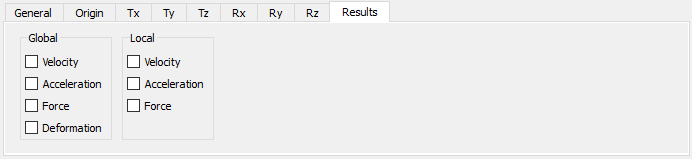
\includegraphics[width=\textwidth]{\ReferenceImg/prp/triad-6}}
    \put(35,55){\Bullet{1}}
    \put(80,55){\Bullet{2}}
  \end{picture}
\end{figure}

The {\sl Results} tab of the Property Editor panel for a Triad (shown
above) contains toggles for activating output of secondary solution
variables to the results database for the triad, such that they are
available for curve plotting, etc.

\begin{bulletlist}
\item{\sl Global} --
  Activates output of quantities measured in the global coordinate system.
  {\sl Deformation} represents the displacement (and rotation) of the triad,
  relative to the rigid body motion of the Part (or Beam) the triad is
  connected to. For triads that are not connected to a Part or a Beam,
  it will be equal to the total displacement of the triad.

\item{\sl Local} --
  Activates output of quantities measured in the local with-rotated coordinate
  system of the triad.
\end{bulletlist}

\Tip{You don't need to enable these toggles if the solver option
  {\tt -allSecondaryVars} or {\tt -allTriadVars} is used.
  Then these quantities will be stored for all triads in the model.}
